\documentclass{beamer}

\usepackage[utf8]{inputenc}
\usepackage{amsmath}
\usepackage{graphicx}
\usepackage{xcolor}
\usepackage{style}
\usepackage[ddmmyyyy]{datetime}
\usepackage{svg}

\title{Kalman Filter}
\subtitle{Grundlagen}
\author{P.Schön, C.Thein}
\date{\today}
\renewcommand{\dateseparator}{.}



\begin{document}

\frame{\titlepage}

\begin{frame}
    \frametitle{Inhaltsverzeichnis}
    \tableofcontents
\end{frame}

\section{Einleitung}

\begin{frame}
    \frametitle{Was ist das Kalman Filter?}
    Das Kalman Filter ist ein mathematisches Verfahren zur iterativen Schätzung von Parametern zur
    Beschreibung von Systemzuständen.

    Dabei wird wiederholt eine Vorhersage über einen Parameterwert
    abgegeben, mit dem fehleranfälligen Messwert kombiniert, und erneut gnutzt um daraus eine Vorhersage
    zu treffen.
\end{frame}

\section{Vereinfachte Erklärung}




\begin{frame}
    \frametitle{Ablauf des Kalman Filters}

    \textbf{Vorhersage}

    1. Denn nächten Zustand darstellen: \( \hat{x}_{k} = A\hat{x}_{k-1}+Bu_{k-1} \)

    2. Die Fehlerkovarianz vorausberechnen: \( P_{k}=AP_{k-1}A^{T}+Q \)

    \textbf{Korrektur}

    3. Den Kalman Gain berechnen: \( K_{k}=P_{k}H^{T}(HP_{k}H^T+R)^{-1} \)

    4. Die Schätzung mit \(z_k\) aktualisieren: \( \hat{x}_{k}=\hat{x}_{k}+K_{k}(z_{k}-H\hat{x}_{k}) \)

    5. Die Fehlerkovarianz aktualisieren: \( P_{k}=(I-K_{k}H)P_{k} \)
\end{frame}


\begin{frame}
    \frametitle{Kalman explained}
    \begin{figure}
        \centering
        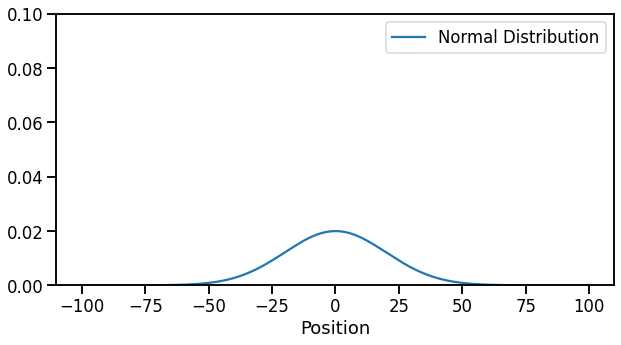
\includegraphics[width=0.7\textwidth]{images/01_normal_distribution.png}
        \caption{Start Postion at \(t_0\)}
    \end{figure}
\end{frame}

\begin{frame}
    \frametitle{Kalman explained}
    \begin{figure}
        \centering
        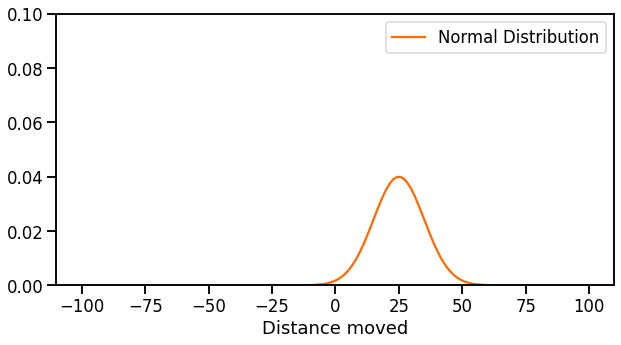
\includegraphics[width=0.9\textwidth]{images/02_normal_distribution_after_move.png}
        \caption{Calculated Postion at \(t_1\)}
    \end{figure}
\end{frame}

\begin{frame}
    \frametitle{Kalman explained}
    \begin{figure}
        \centering
        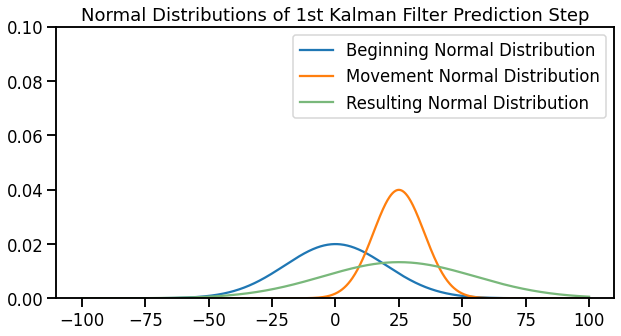
\includegraphics[width=0.9\textwidth]{images/03_first_prediction.png}
        \caption{Predicted Postion at \(t_1\)}
    \end{figure}
\end{frame}

\begin{frame}
    \frametitle{Kalman explained}
    \begin{figure}
        \centering
        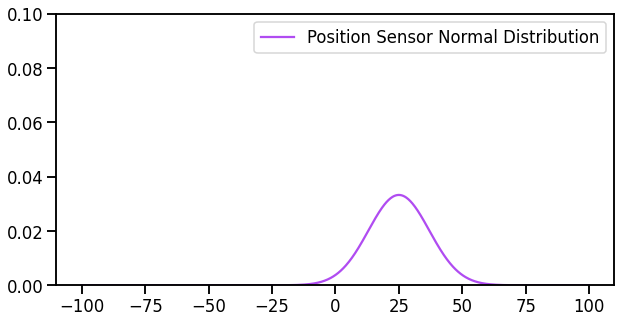
\includegraphics[width=0.9\textwidth]{images/04_measurement.png}
        \caption{Messured Sensor Data of Postion at \(t_1\)}
    \end{figure}
\end{frame}

\begin{frame}
    \frametitle{Kalman explained}
    \begin{figure}
        \centering
        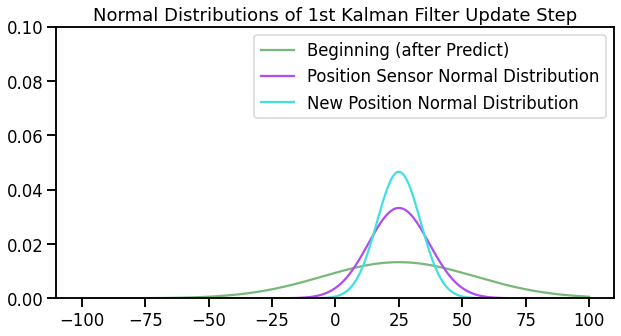
\includegraphics[width=0.9\textwidth]{images/05_correction.png}
        \caption{Correction of the Kalman Gain after Messurement at \(t_1\)}
    \end{figure}
\end{frame}

\begin{frame}
    \frametitle{Takeaways}
    \begin{itemize}
        \item The precision sinks with the prediction
        \item The precision grows with the correction
    \end{itemize}
    
\end{frame}

\section{Joystick example}

\begin{frame}
    \frametitle{State Representation}
    % //TODO: Make x's differentiabable
    We define the state vector \(x\) to include the position and velocity of the mouse in both x and y directions
    \[
        \left[ \begin{array}{r}
            x  \\
            y  \\
            v_{x}  \\
            v_{y} \\
        \end{array}\right]    
    \]
    where:
    \begin{itemize}
        \item \(x\) is the position on the x-axis
        \item \(y\) is the postion on the y-axis
        \item \(v_{x}\) is the velocity in the x-direction
        \item \(v_{y}\) is the velocity in the y-direction

    \end{itemize}
\end{frame}

\begin{frame}
    \frametitle{Formulate the Transtition Model}
    The state transition model describes how the state evolves from one time step to the next. 
    If we assume a constant velocity model, the state transition can be expressed as:
    \[x_{k+1}=Ax_{k}+w_{k}\]
    where \(w_{k}\) represents the proces noise, assumed to be Gaussian with zero mean and covariance \(Q\).
\end{frame}

\begin{frame}
    \frametitle{Create the Transition Matrix}
    % //TODO: Adjust Velocity to not be constant
    The transition matrix A for a constant velocity Model is: 
    \[
        \left[ \begin{array}{rrrr}
            1 & 0 & \Delta t & 0        \\
            0 & 1 & 0        & \Delta t \\
            1 & 0 & 1        & 0        \\
            0 & 0 & 0        & 1        \\
        \end{array}\right]    
    \]
    \(\Delta t\) is the time intervall between mesurements.
\end{frame}

\begin{frame}
    \frametitle{Observation Model}
    The observation model realtes the state to the measurements:
    \[z_{k}=Hx_{k}+v_{k}\]
    where \(v_{k}\) represents the measurement noise, assumed to be Gaussian with zero mean and
    covariance \(R\).

    The observation matrix \(H\) for direct measurement of position is:
    \[H = \left[
        \begin{array}{rrrr}
            1 & 0 & 0 & 0 \\
            0 & 1 & 0 & 0 \\
        \end{array}
    \right]\]
\end{frame}

\begin{frame}
    \frametitle{Prediction Step}
    The prediction step estimates the next state and its uncertainty:
    \begin{itemize}
        \item Predict the state:
    \end{itemize}
    \[x_{k+1}=Ax_{k}\]
    \begin{itemize}
        \item Predict the error coavriance:
    \end{itemize}
    \[P_{k+1}=AP_{k}A^{T}+Q\]
\end{frame}

\begin{frame}
    \frametitle{Correction Step}
    The correction step updates the state estimate with the new measurement:
    \begin{itemize}
        \item Compute the Kalman gain:
    \end{itemize}
    \[K_{k} = P_{k}H^{T}(HP_{k}H^{T}+R)^{-1}\]
    \begin{itemize}
        \item Update the state estimate:
    \end{itemize}
    \[x_{k} = x_{k}+K_{k}(z_{k}-Hx_{k})\]
    \begin{itemize}
        \item Update the error covariance:
    \end{itemize}
    \[P_{k} = (I-K_{k}H)P_{k}\]
\end{frame}

\begin{frame}
    \frametitle{Kalman Filter}
    \begin{figure}
        \centering
        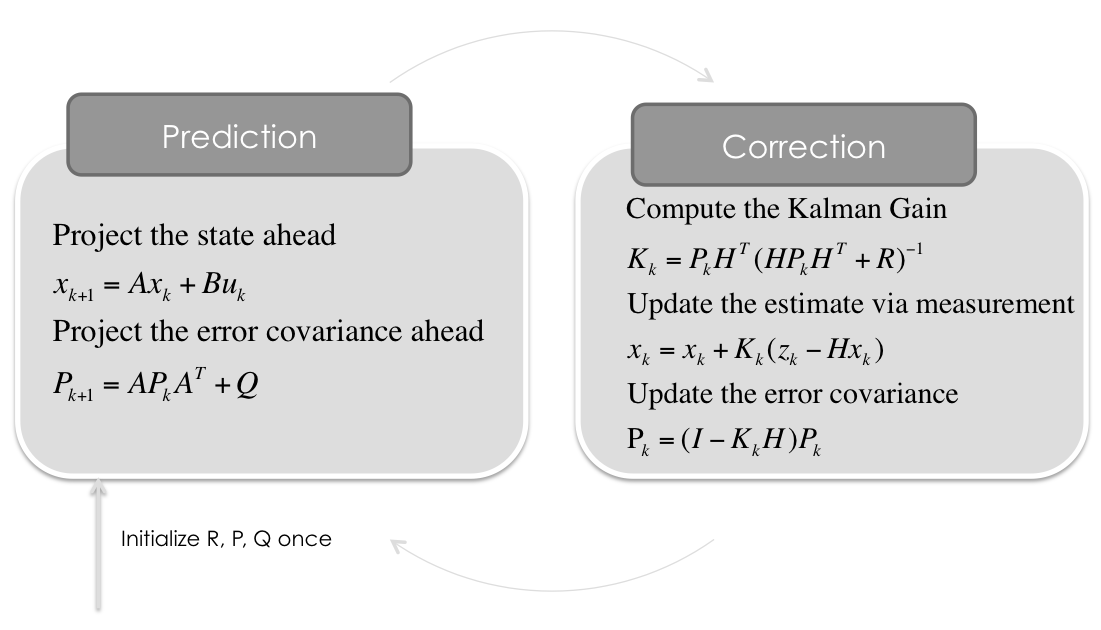
\includegraphics[width=0.95\textwidth]{images/06_kalman_diagram.png}
        \caption{Iterative Nature of the Kalman filter}
    \end{figure}
\end{frame}

\begin{frame}
    \frametitle{Cheat Sheet - Math Symbols}
    \begin{table}[h]
        \centering
        \begin{tabular}{|c|p{8cm}|}
        \hline
        \textbf{Zeichen} & \textbf{Bedeutung} \\ \hline
        k          & Zeitintervall der Messwerte / Iteration \\ \hline
        z\_k       & gemessene Geschwindigkeit des Sensors \\ \hline
        x\_k       & Wert der aktuellen Schätzung \\ \hline
        x\_{k-1}   & Wert der vorherigen Schätzung \\ \hline
        P\_k       & Wert der aktuellen Fehlerkovarianz \\ \hline
        P\_{k-1}   & Wert der vorherigen Fehlerkovarianz \\ \hline
        R          & Varianz der Messergebnisse \\ \hline
        Q          & Process noise covariance \\ \hline
        A          & Transition Matrix \\ \hline
        H          & Observation Matrix \\ \hline
        B*u\_{k-1} & Control signal \\ \hline
        \end{tabular}
        \end{table}
\end{frame}

\section{EXAMPLES}

\begin{frame}
    \frametitle{Ablauf des Kalman Filters}
    \begin{itemize}
        \item \textbf{Fettgedruckt}
        \item \textit{Kursiv}
        \item \underline{Unterstrichen}
        \item \texttt{Monospaced}
    \end{itemize}
\end{frame}

\begin{frame}
    \frametitle{Aufzählungen}
    \begin{itemize}
        \item Erster Punkt
        \item Zweiter Punkt
        \item Dritter Punkt
    \end{itemize}
\end{frame}

\begin{frame}
    \frametitle{Mathematische Ausdrücke}
    \begin{itemize}
        \item Inline: \(E = mc^2\)
        \item Displayed:
              \[
                  \int_0^\infty e^{-x^2} \, dx = \frac{\sqrt{\pi}}{2}
              \]
    \end{itemize}
\end{frame}

\begin{frame}
    \frametitle{Bilder einfügen}
    \begin{figure}
        \centering
        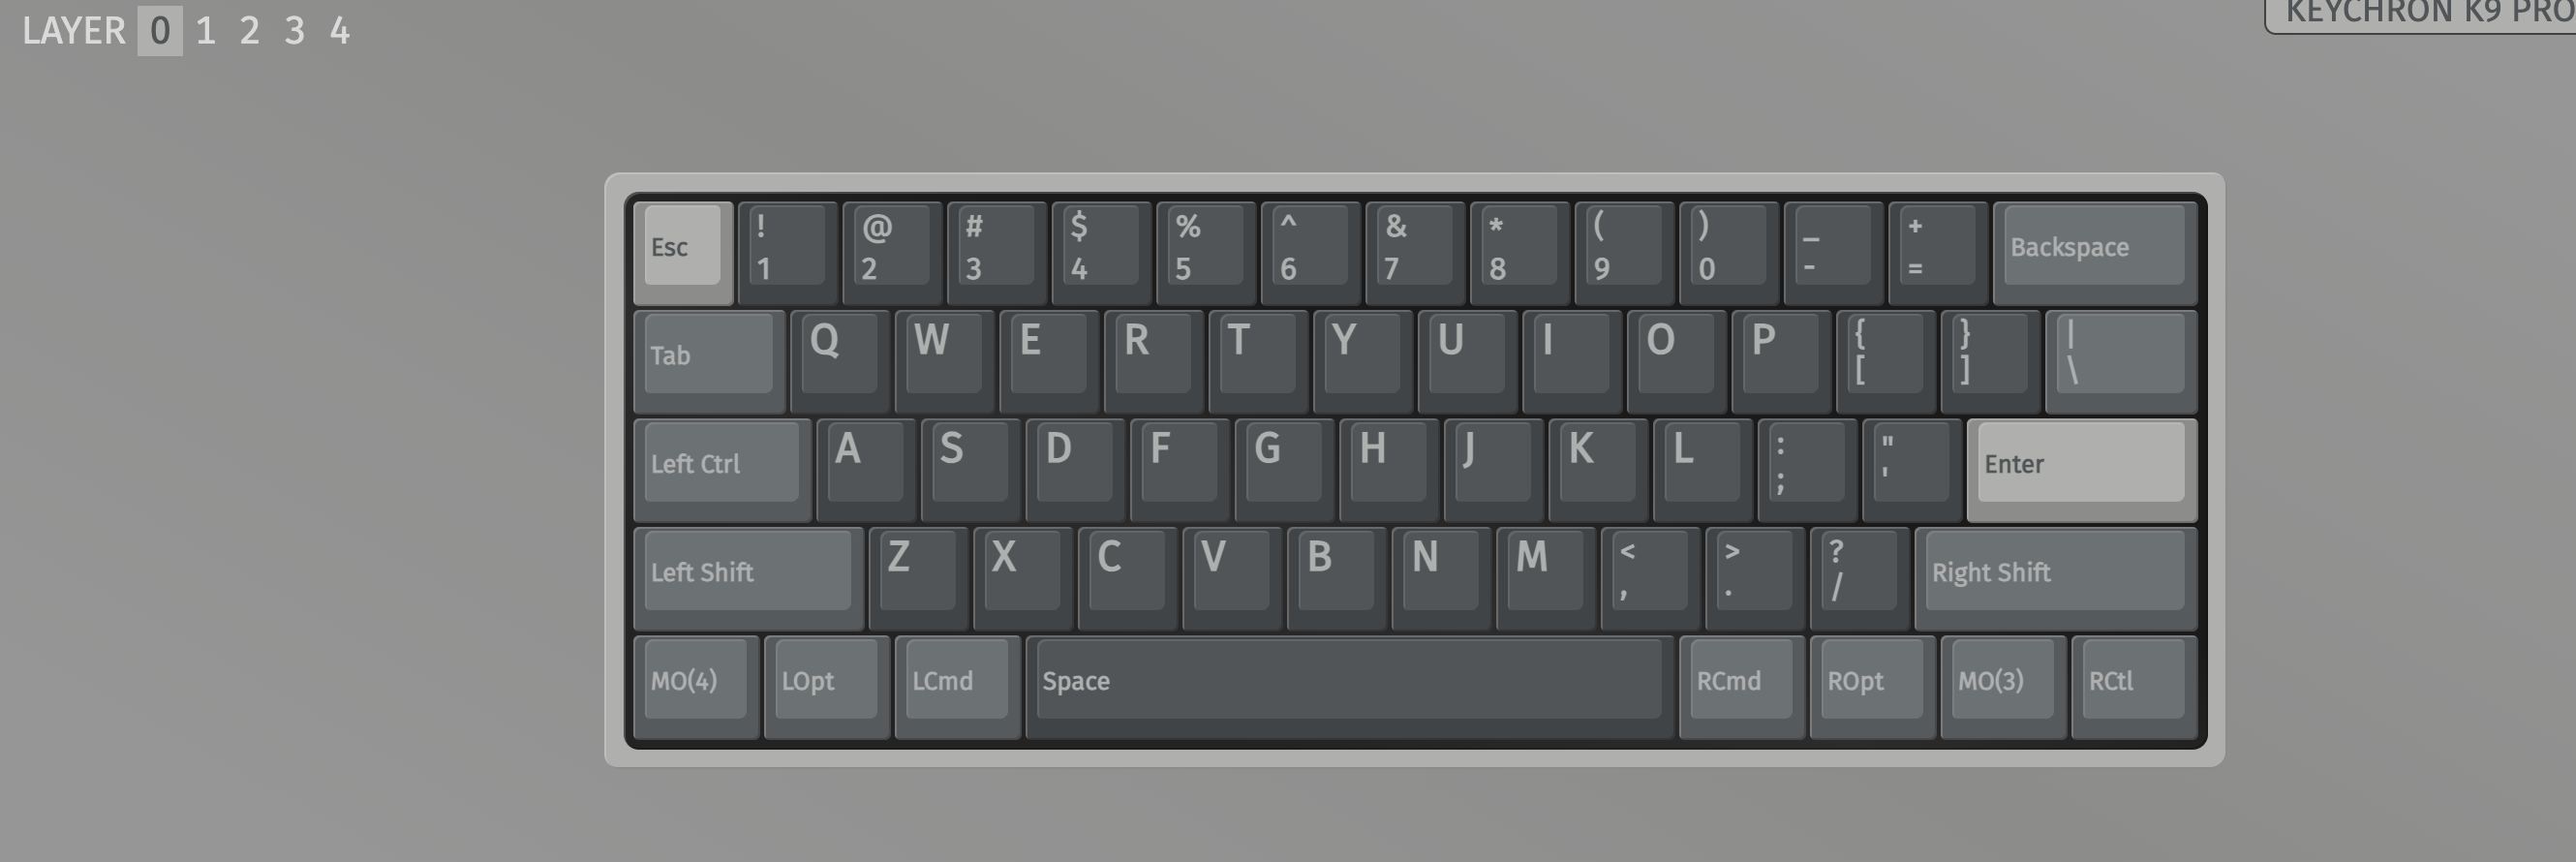
\includegraphics[width=0.5\textwidth]{sample}
        \caption{Ein Beispielbild}
    \end{figure}
\end{frame}

\section{Zusammenfassung}

\begin{frame}
    \frametitle{Zusammenfassung}
    In dieser Präsentation haben wir die grundlegenden Elemente von LaTeX vorgestellt, darunter:
    \begin{itemize}
        \item Textformatierung
        \item Aufzählungen und Listen
        \item Mathematische Ausdrücke
        \item Bilder einfügen
    \end{itemize}
\end{frame}

\end{document}
\ProvidesPackage{beamerthemesss}
\mode<presentation>
\usepackage{xcolor}
\usepackage{tikz}
\RequirePackage{enumitem} 


\definecolor{orange_100}{RGB}{255, 107, 0} 	% orange_100
\definecolor{orange_80}{RGB}{255, 137, 51} 	% orange_80
\definecolor{black_100}{RGB}{0, 0, 0} 		% black_100
\definecolor{black_80}{RGB}{50, 50, 50} 		% black_80
\definecolor{black_60}{RGB}{100, 100, 100} 	% black_60
\definecolor{white}{RGB}{255, 255, 255} 		% white


% Define a command to set the foreground color of lists
\newcommand{\setlistcolor}[1]{
    \setlist[enumerate]{label=\textcolor{#1}{\textbullet}}
    \setlist[itemize]{label=\textcolor{#1}{\textbullet}}
}
\setlistcolor{orange_80}

% Schriftarten einstellen
\setbeamerfont{title}{size=\huge,series=\bfseries}
\setbeamerfont{subtitle}{size=\small,series=\bfseries}
\setbeamerfont{frametitle}{size=\large,series=\bfseries}
\setbeamerfont{normal text}{size=\small}

% Farben anwenden
\setbeamercolor{title}{fg=orange_100}
\setbeamercolor{subtitle}{fg=black_60}
\setbeamercolor{frametitle}{fg=orange_100}
\setbeamercolor{section in toc}{fg=black_80}
\setbeamercolor{normal text}{fg=black_80}
\renewcommand{\figurename}{\textcolor{orange_100}{Fig.}}

% Layout anpassen
\setbeamertemplate{navigation symbols}{}

% Customize header and footer with dotted lines made of circles
\setbeamertemplate{headline}{
    \begin{tikzpicture}[remember picture,overlay]
    	\ifnum\theframenumber=1
        \node[anchor=north east, inner sep=0pt, yshift=-0.5mm, xshift=-2mm] at (current page.north east) {
            
\includegraphics[height=4.8mm]{logo.png}
        };
        \fi
        \draw[thick, dash pattern=on 0pt off 2\pgflinewidth, line cap=round, color=orange_100]
              ([yshift=-7.5mm]current page.north west) -- 
              ([yshift=-7.5mm]current page.north east);
    \end{tikzpicture}
}

\setbeamertemplate{footline}{
    \begin{tikzpicture}[remember picture,overlay]
        \ifnum\theframenumber>1
        	\draw[thick, dash pattern=on 0pt off 2\pgflinewidth, line cap=round, color=orange_100] 
              ([yshift=8mm]current page.south west) -- 
              ([yshift=8mm]current page.south east);
                      \node[anchor=east, inner sep=0pt, yshift=2.5mm, xshift=-5mm] at (current page.south east) {
        					\color{black_60}
        					\insertframenumber/
        					\inserttotalframenumber
        	};
        	\node[anchor=west, inner sep=0pt, yshift=3.5mm, xshift=-2mm] at (current page.south west) {
        		
\includegraphics[height=7.8mm]{watermark.png}
        	};
        \fi
        \ifnum\theframenumber=1
        	\node[anchor=west, inner sep=0pt, yshift=6mm, xshift=-4mm] at (current page.south west) {
        		
\includegraphics[height=9.8mm]{watermark.png}
        	};
        \fi

    \end{tikzpicture}
}

% Abschnittsüberschriften
\setbeamercolor{section in head/foot}{bg=orange_100,fg=white}
\setbeamerfont{section in head/foot}{series=\bfseries}
\setbeamertemplate{section in head/foot shaded}{\color{orange_100!50}}

\setbeamertemplate{frametitle}{
    \begin{tikzpicture}[remember picture,overlay]
        \node[
        	anchor=base west, 
        	fill=white, 
        	yshift=-3.9mm, 
        	xshift=-2mm
        ] {\bfseries\insertframetitle};
    \end{tikzpicture}
}


\endinput

